\chapter{Grundlagen}
\section{Git Repository anlegen}
\subsection{Existierendes Verzeichnis initialisieren}
Ein bereits existierendes Verzeichnis kann als Git Repository initialisiert werden. Dabei wird ein Unterverzeichnis \texttt{.git} angelegt. Bereits im Verzeichnis erhaltene Daten werden nicht automatisch versioniert. Dies geschieht mit dem ersten Commit.\\
\begin{lstlisting}[caption={Initialisierung},captionpos=b]
git init
\end{lstlisting}
\subsection{Existierendes Repository klonen}
Um eine Kopie eines existierenden Projekts zu erstellen wird dieses geklont. Alle bereits vorhandenen Daten werden als lokale Kopie des Projekts gespeichert. Dabei wird ein Verzeichnis mit dem Namen des Projekts angelegt.\\
\begin{lstlisting}[caption={Clone},captionpos=b]
git clone [url]

#Eigener Verzeichnisname
git clone [url] newDir
\end{lstlisting}
\section{Änderungen nachverfolgen}
Dateien im Arbeitsverzeichnis können entweder verfolgt (tracked) oder nicht verfolgt (untracked) werden. Alle Dateien des letzten Commits befinden sich in der Versionskontrolle. Diese Dateien können unverändert (unmodified), verändert (modified) oder für den nächsten Commit vorgemerkt (staged) vorliegen. Alle anderen Dateien sind nicht versioniert (Nicht im letzten Commit und nicht in der Staging Area).
\begin{figure}[H]
	\centering
		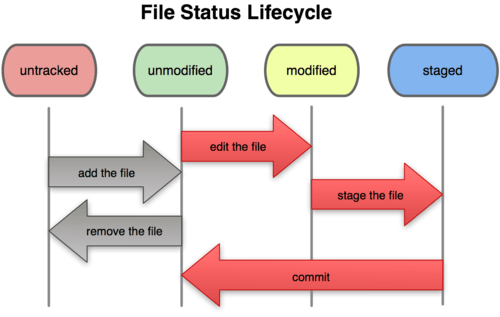
\includegraphics[width=0.6\textwidth]{img/follow.png}
	\caption{File Status LC}
\end{figure}
\section{Status prüfen}
\begin{lstlisting}[caption={Status},captionpos=b]
git status
\end{lstlisting}
\section{Dateien hinzufügen}
\begin{lstlisting}[caption={Add},captionpos=b]
git add newFile
\end{lstlisting}
\section{Dateien stagen}
\begin{lstlisting}[caption={Stage},captionpos=b]
git add existingFile
\end{lstlisting}
\section{Dateien ignorieren}
In der Datei \texttt{.gitignore} können Regeln hinterlegt werden, welche Dateien von Git ignoriert werden sollen.
\section{Staging Area durchsuchen}
Um die Staging Area und das Arbeitsverzeichnis direkt zu vergleichen kann \texttt{diff} benutzt werden.
\begin{lstlisting}[caption={Diff},captionpos=b]
git diff
\end{lstlisting}
\section{Commit aus Staging Area erzeugen}
\begin{lstlisting}[caption={Commit},captionpos=b]
#Editor
git commit

#Editor mit diff
git commit -v

#Meldung direkt angeben
git commit -m ''Message from Hell''
\end{lstlisting}
\section{Staging Area überspringen}
Alle Dateien, welche sich bereits unter Versionskontrolle befinden, werden im Commit aufgenommen.
\begin{lstlisting}[caption={Commit w/o Staging Area},captionpos=b]
git commit -a
\end{lstlisting}
\section{Dateien entfernen}
\subsection{Staging Area}
\begin{lstlisting}[caption={RM Staging Area},captionpos=b]
git rm --cached file.txt
\end{lstlisting}
\subsection{Arbeitsverzeichnis}
\begin{lstlisting}[caption={RM},captionpos=b]
#delete file
rm file.txt
#staging area
git rm file.txt
#commit
git commit
\end{lstlisting}
\section{Dateien verschieben}
Git verfolgt nicht explizit, ob Dateien verschoben werden.
\begin{lstlisting}[caption={Move},captionpos=b]
git move file_from file_to
\end{lstlisting}
\section{Historie}
Der Befehl \texttt{git log} listet alle Commits eines Projekts in umgekehrter chronologischer Reihenfolge auf. Mit Hilfe von Optionen kann bestimmt werden, welche Informationen angezeigt werden sollen.\\
\begin{lstlisting}[caption={Log},captionpos=b]
#normal
git log

#display changes (diff)
git log -p

#diff by words not lines
git log -p --word-diff

#statistc
git log --stat

#one commit per line
git log --pretty=online

#branch graph
git log --pretty=oneline --graph
\end{lstlisting}
\begin{center}
\renewcommand{\arraystretch}{1.2}
\begin{tabular}{|p{4cm}p{10cm}|}
\hline
\textbf{Option}				&\textbf{Beschreibung}\\
\hline
\texttt{-p}					&Zeigt Patch eines Commits\\
\hline
\texttt{-{}-word-diff}			&Vergleich Wort zu Wort\\
\hline
\texttt{-{}-stat}				&Statistik der geänderten Dateien und entfernten/hinzugefügten Zeilen\\
\hline
\texttt{-{}-startstat}			&Kurzstatistik über eingefügte/entfernte Zeilen\\
\hline
\texttt{-{}-name-only}			&Liste der geänderten Dateienen nach Commit Informationen\\
\hline
\texttt{-{}-name-status}		&Liste der Dateien mit hinzufügt/geändert/entfernt Statistik\\
\hline
\texttt{-{}-abbrev-commit}		&Zeigt nur erste Zeichen einer SHA-1 Checksum\\
\hline
\texttt{-{}-relative-date}		&Zeigt Datum in relativen Format\\
\hline
\texttt{-{}-graph}				&ASCII Graph der Branch- und Merch-Historie\\
\hline
\texttt{-{}-pretty}				&Zeigt Commits in alternativen Format (online, short, full, fuller und format [eigenes Format spezifizieren])\\
\hline
\end{tabular}
\captionof{table}{Log Options Format}
\renewcommand{\arraystretch}{1}
\end{center}
\newpage
\subsection{Log Dateien Filtern}
Außerdem stehen weitere Optionen zur Verfügung, die zur Filterung der Ergebnisse dienen.
\begin{center}
\renewcommand{\arraystretch}{1.2}
\begin{tabular}{|p{4cm}p{10cm}|}
\hline
\textbf{Option}				&\textbf{Beschreibung}\\
\hline
\texttt{-(n)}					&Ausgabe von n Commits\\
\hline
\texttt{-{}-since, -{}-after}		&Commits nach dem angegebenen Datum\\
\hline
\texttt{-{}until, -{}-before}		&Commits vor dem angegebenen Datum\\
\hline
\texttt{-{}-author}			&Commits von angegebenen Author\\
\hline
\texttt{-{}-committer}			&Commits vcon angegebenen Committer\\
\hline
\texttt{-{}-no-merges}			&Commits welche keine Merges sind\\
\hline
\end{tabular}
\captionof{table}{Log Options Format}
\renewcommand{\arraystretch}{1}
\end{center}
\section{Änderungen rückgängig machen}
\subsection{letzten Commit ändern}
Ändert den letzten Commit (vergessene Dateien hinzufügen, Message ändern). Direkt nach dem letzten Commit auszuführen, wenn noch keine weiteren Änderungen gemacht wurden (Staging Area wird verwendet).\\
\begin{lstlisting}[caption={letzten Commit ändern},captionpos=b]
#texteditor new message
git commit --amend

#add forgotten file
git commit -m 'initial commit'
git add forgotten_file
git commit --amend
\end{lstlisting}
\subsection{Änderungen aus Staging Area entfernen}
\begin{lstlisting}[caption={Entfernen aus Staging Area},captionpos=b]
#list files in staging area
git status

#remove file from staging area
git reset HEAD <file>
\end{lstlisting}
\subsection{Änderungen an einer Datei rückgängig machen}
\begin{lstlisting}[caption={Änderungen an Datei rückgängig machen},captionpos=b]
#file status last commit
git checkout -- <file>
\end{lstlisting}
\section{Externe Repositorys}
\subsection{Remote Repositorys anzeigen}
\begin{lstlisting}[caption={Repo anzeigen},captionpos=b]
#display remote server
git remote

#display remote server with url
git remote -v
\end{lstlisting}
\subsection{Remote Repository hinzufügen}
\begin{lstlisting}[caption={Repo hinzufügen},captionpos=b]
#add repo with shortname
git remote add [shortname] [url]
\end{lstlisting}
\subsection{Änderunges aus Remote Repository herunterladen und zusammenführen}
\begin{lstlisting}[caption={Repo zusammenführen},captionpos=b]
#download changes without merging
git fetch [remote-name]

#download changes with merging (only if branch tracked)
git pull
\end{lstlisting}
\subsection{Änderunges hochladen}
\begin{lstlisting}[caption={Änderungen hochladen},captionpos=b]
#upload changes
git push [remote-name] [branch-name]
\end{lstlisting}
\subsection{Repository ansehen}
\begin{lstlisting}[caption={Repository ansehen},captionpos=b]
#display remote repository
git remote show [remote-name]
\end{lstlisting}
\subsection{Verweise auf Remote Repository}
\begin{lstlisting}[caption={Verweise auf Remote Repo},captionpos=b]
#rename
git remote rename name newName

#remove
git remote rm name
\end{lstlisting}
\section{Tags}
\subsection{Tags anzeigen}
\begin{lstlisting}[caption={Tags anzeigen},captionpos=b]
#display tags alphabetical
git tag

#display only versions that belong to 1.x
git tag -l 'v.1.*'
\end{lstlisting}
\subsection{Tags anlegen}
Git bietet zwei verschiedene Typen von Tags an. einfache Tags (lightweight) und kommentierte (annotated) Tags. Ein einfacher Branch ist ein Zeiger auf einen bestimmten Commit. Kommentierte Tags werden als Objekte in Git gespeichert.\\
\begin{lstlisting}[caption={Tags anlegen (Teil 1)},captionpos=b]
#lightweight tag
git tag v1.0

#annotated tag
git tag -a v1.0

#annotated tag with message
git tag -a v1.0 -m 'first release version'

#annotated GPG signed tag with message
git tag -s v1.0 -m 'first release version'

#verify signed tag
git tag -v [tagname]

#display tag
git show [tagname]
\end{lstlisting}
\newpage
\begin{lstlisting}[caption={Tags anlegen (Teil 2)},captionpos=b]
#tag afterwards
git tag -a [tagname] -m [message] [hash]

#upload tag
git push origin [tagname]

#upload all tags
git push origin --tags
\end{lstlisting}
\section{Auto-Vervollständigung}
Mit Hilfe eines Bash Scriptes ist es möglich eine Auto-Vervollständigung für die Bash auf Linux Systemen einzurichten. Das Script kann von folgender Quelle bezogen werden: \\
\texttt{https://github.com/git/git/blob/master/contrib/completion/git-completion.bash }
Im Verzeichnis \texttt{/etc/bash\_completion.d/} ist nun eine Datei mit dem Namen\newline
\texttt{git-completion.bash} anzulegen. Mit \texttt{Tab} kann nun die Autovervollständigung erfolgen (2 mal drücken für Vorschläge).
\section{Git Aliase}
In Git können Aliase dazu verwendet werden um häufig verwendete Befehle abzukürzen.\\
\begin{lstlisting}[caption={Alias},captionpos=b]
git config --global alias.[name] [befehl]
\end{lstlisting}